\label{Static Routing}
\chapter{Linux PC Configuration as a simple IP router}
In this section we are going to set up configuration of a Linux PC as a simple IP router with two network interface
\begin{figure}[H]
\centering
  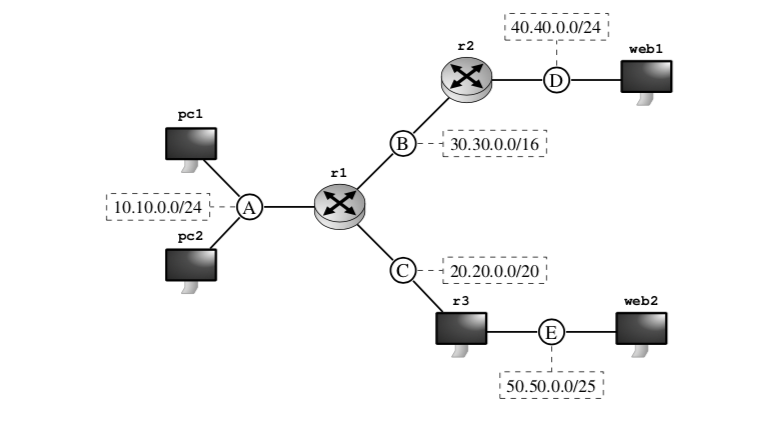
\includegraphics[width=400pt]{Images/1.assignment.02.png}
  \caption{Linux PC as IP Router}
  \label{fig:2.33}
\end{figure}
\section{Lab.conf File}
\begin{figure}[H]
\centering
  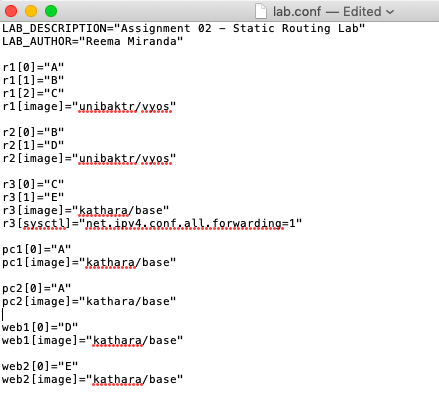
\includegraphics[width=300pt]{Images/lab_static_routing.conf.png}
  \caption{Lab.Conf File}
  \label{fig:2.1}
\end{figure}
\subsection{Creating the four devices}
\subsection{Creating 2 PCs ,2 web devices and 3 routers each assigned a network interface and unique collision domain}
\paragraph{}
   1.kathara lstart: to start the lab file where all machines are created simultaneously.
\begin{figure}[H]
\centering
  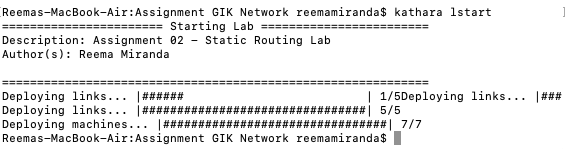
\includegraphics[width=400pt]{Images/kathara lstart.png}
  \caption{Created 2 PCs ,2 web devices,3 routers each assigned a network interface with unique collision domain}
<<<<<<< HEAD
  \label{fig:2.2}
\end{figure}
\section{Docker Image}
\paragraph{}
docker ps:To check docker images for each container
 \begin{figure}[H]
\centering
  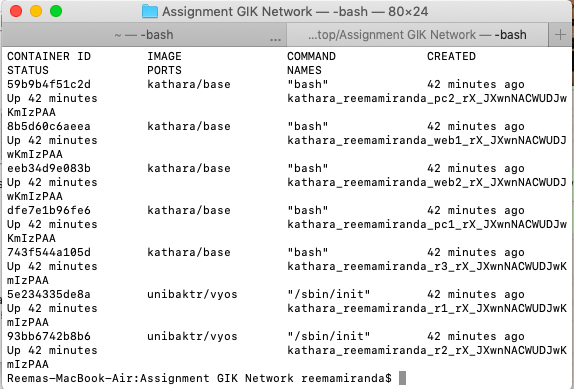
\includegraphics[width=400pt]{Images/docker ps.png}
  \caption{Image Ports for each Machine}
  \label{fig:2.3}
\end{figure}
\subsection{Startup Files}
\begin{figure}[H]
\centering
  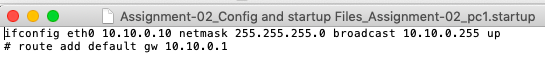
\includegraphics[width=400pt]{Images/PC1.startup.png}
  \caption{PC1.startup file}
  \label{fig:2.4}
\end{figure}
\begin{figure}[H]
\centering
  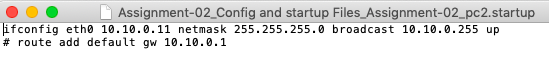
\includegraphics[width=400pt]{Images/pc2.startup.png}
  \caption{PC2.startup file}
  \label{fig:2.5}
\end{figure}
\begin{figure}[H]
\centering
  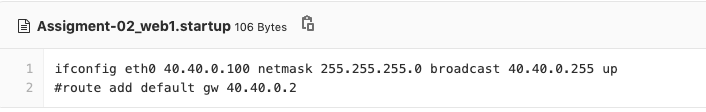
\includegraphics[width=400pt]{Images/web1.startup.png}
  \caption{web1.startup file}
  \label{fig:2.6}
\end{figure}
\begin{figure}[H]
\centering
  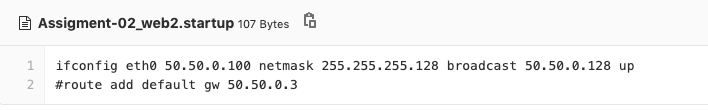
\includegraphics[width=400pt]{Images/web2.startup.png}
  \caption{web2.startup file}
  \label{fig:2.7}
\end{figure}
\begin{figure}[H]
\centering
  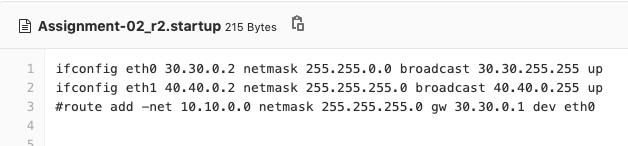
\includegraphics[width=400pt]{Images/r2.startup.png}
  \caption{r2.startup file}
  \label{fig:2.8}
\end{figure}
\begin{figure}[H]
\centering
  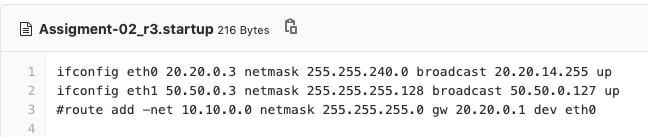
\includegraphics[width=400pt]{Images/r3.startup.png}
  \caption{r3.startup file}
  \label{fig:2.9}
\end{figure}
\begin{figure}[H]
\centering
  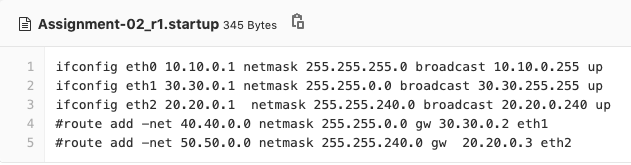
\includegraphics[width=400pt]{Images/r1.startup.png}
  \caption{r1.startup file}
  \label{fig:2.10}
=======
  \label{fig:3.2}
\end{figure}
\section{Docker Image}
\paragraph{}
docker ps:To check docker images for each container
 \begin{figure}[H]
\centering
  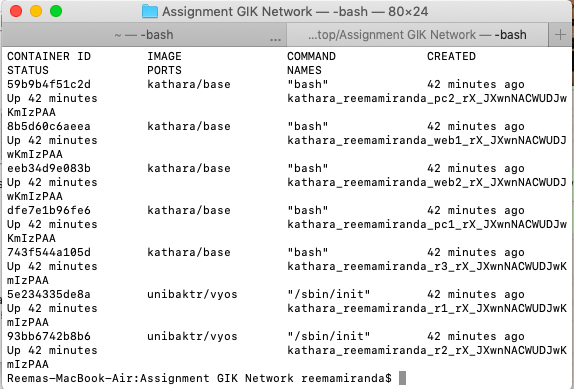
\includegraphics[width=400pt]{Images/docker ps.png}
  \caption{Image Ports for each Machine}
  \label{fig:3.4}
\end{figure}
\subsection{Startup Files}
\begin{figure}[H]
\centering
  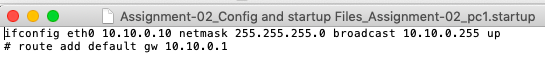
\includegraphics[width=400pt]{Images/PC1.startup.png}
  \caption{PC1.startup file}
  \label{fig:3.2}
\end{figure}
\begin{figure}[H]
\centering
  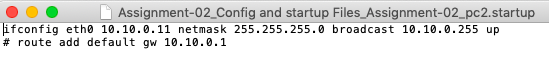
\includegraphics[width=400pt]{Images/pc2.startup.png}
  \caption{PC2.startup file}
  \label{fig:3.2}
\end{figure}
\begin{figure}[H]
\centering
  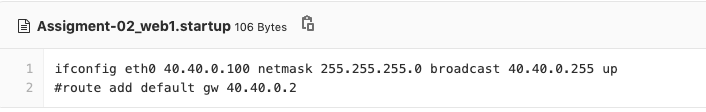
\includegraphics[width=400pt]{Images/web1.startup.png}
  \caption{web1.startup file}
  \label{fig:3.2}
\end{figure}
\begin{figure}[H]
\centering
  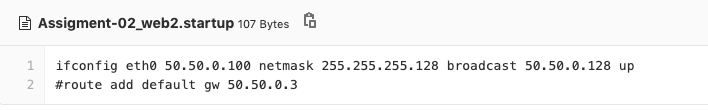
\includegraphics[width=400pt]{Images/web2.startup.png}
  \caption{web2.startup file}
  \label{fig:3.2}
\end{figure}
\begin{figure}[H]
\centering
  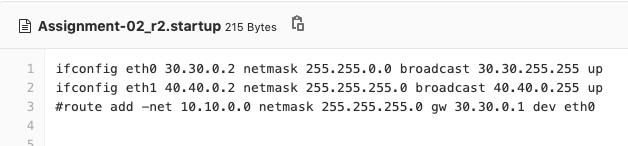
\includegraphics[width=400pt]{Images/r2.startup.png}
  \caption{r2.startup file}
  \label{fig:3.2}
\end{figure}
\begin{figure}[H]
\centering
  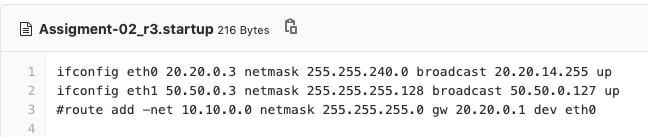
\includegraphics[width=400pt]{Images/r3.startup.png}
  \caption{r3.startup file}
  \label{fig:3.2}
\end{figure}
\begin{figure}[H]
\centering
  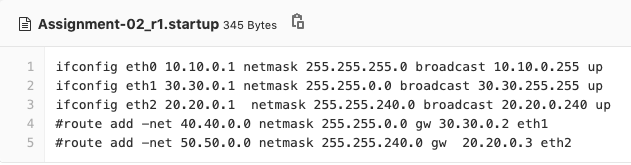
\includegraphics[width=400pt]{Images/r1.startup.png}
  \caption{r1.startup file}
  \label{fig:3.2}
>>>>>>> 48a684cd851a8df39224f8b6725a51314ead5f6e
\end{figure}
\section{Configuring the four devices}
\paragraph{}
The purpose of using subnetting is to reduce the traffic congestion.
\\Ex:pc1 and pc2 connect to same router r1 over the same interface eth0.As both send packets to router r1 there will be traffic congestion and also the speed of the network reduces .Hence we are subnetting the IP address.
\subsection{Configuring an IP address for PC1,PC2,Web1 and Web2 }
 \begin{figure}[H]
\centering
  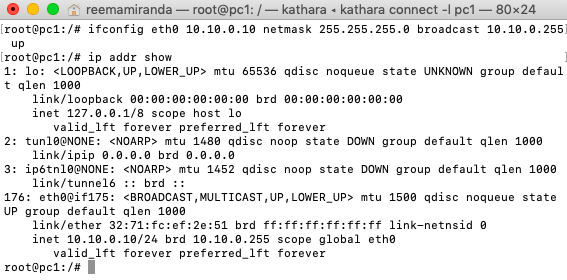
\includegraphics[width=400pt]{Images/pc1.ip.png}
  \caption{configured IP address for PC1}
  \label{fig:2.11}
\end{figure}
\begin{figure}[H]
\centering
  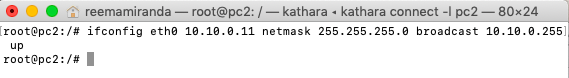
\includegraphics[width=400pt]{Images/pc2.ip.png}
  \caption{configured IP address for PC2}
  \label{fig:2.12}
\end{figure}
\begin{figure}[H]
\centering
  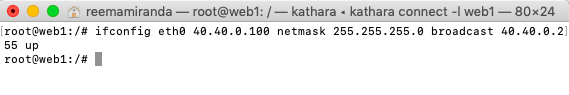
\includegraphics[width=400pt]{Images/web1.ip.png}
  \caption{configured IP address for web1}
  \label{fig:1.13}
\end{figure}
\begin{figure}[H]
\centering
  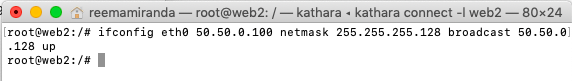
\includegraphics[width=400pt]{Images/web2.ip.png}
  \caption{configured IP address for web2}
  \label{fig:2.14}
\end{figure}
\subsection{Configuring an IP address for R1 ,R2 and R3 routers }
 \begin{figure}[H]
\centering
  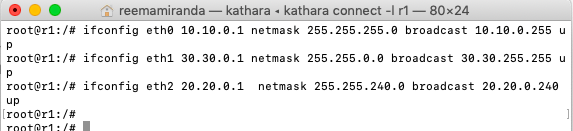
\includegraphics[width=400pt]{Images/r1.ip.png}
  \caption{configured IP address for R1}
  \label{fig:2.15}
\end{figure}
\begin{figure}[H]
\centering
  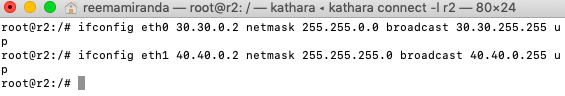
\includegraphics[width=400pt]{Images/r2_ip.png}
  \caption{configured IP address for R2}
  \label{fig:2.16}
\end{figure}
\begin{figure}[H]
\centering
  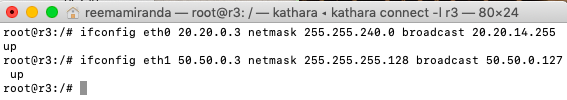
\includegraphics[width=500pt]{Images/r3.ip.png}
  \caption{configured IP address for R3}
  \label{fig:2.17}
\end{figure}
\subsection{Configuring default gateway to reach other networks }
 \begin{figure}[H]
\centering
  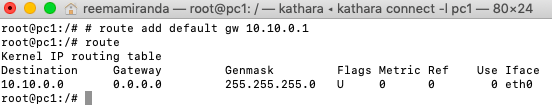
\includegraphics[width=400pt]{Images/pc1_gateway.png}
  \caption{Default gateway for PC1}
  \label{fig:2.18}
\end{figure}
\paragraph{}
In order to establish connection between host on different network we must add the default route. 
Ex: To ping from pc1 to web1 which are on different network interface we must add default route(gateway) from pc1 to r1.Through this gateway(ip address) we can reach other  networks 
<<<<<<< HEAD
\begin{figure}[H]
=======
\begin{figure}
>>>>>>> 48a684cd851a8df39224f8b6725a51314ead5f6e
\centering
  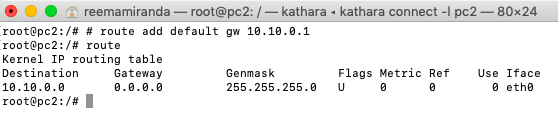
\includegraphics[width=400pt]{Images/pc2_gateway.png}
  \caption{Default gateway for PC2}
  \label{fig:2.19}
\end{figure}
\begin{figure}
\centering
  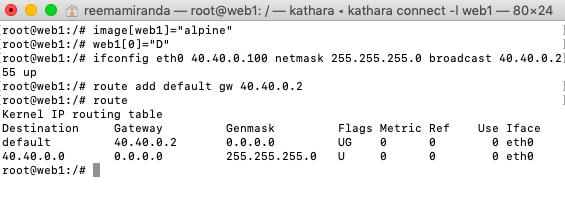
\includegraphics[width=400pt]{Images/web1_gateway.png}
  \caption{Default gateway for Web1}
  \label{fig:2.20}
\end{figure}
\begin{figure}
\centering
  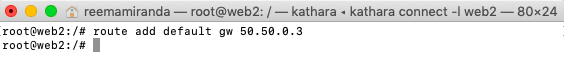
\includegraphics[width=400pt]{Images/web2_gateway.png}
  \caption{Default gateway for Web2}
  \label{fig:2.21}
\end{figure}


\section{Capturing the traffic on the collision domains}
In mac OS we cannot find collision domains in the traffic using Wireshark. To capture the traffic, used ping command to connect to between the systems, and ran tcpdump in the background, and redirected the dump to a .pcap file. Later by importing the .pcap into Wireshark we could able to observe the traffic.
\newline Below screenshots displays the traffic captured from different systems at collision domains,
\subsection{Traffic from pc1 to web1}
Traffic is captured when we ping web1 from pc1 using tcpdump and the .pcap file is imported into the wireshark to display the traffic flow.
\begin{figure}[H]
\centering
  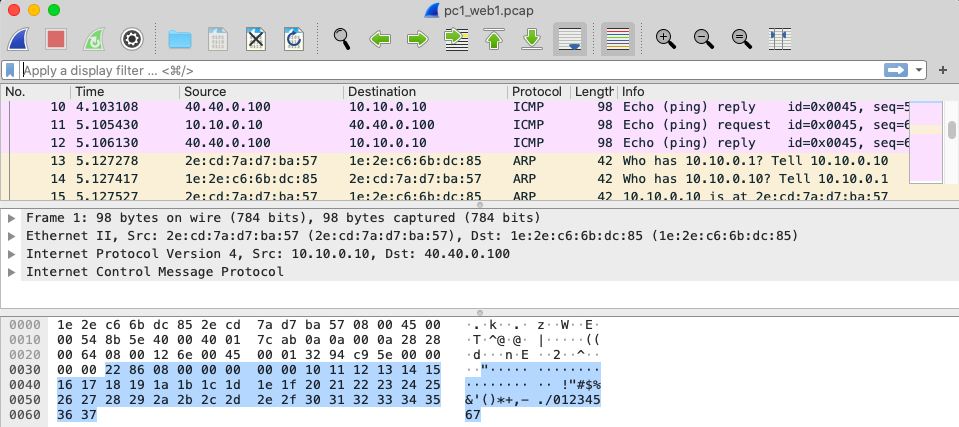
\includegraphics[width=400pt]{Images/pc1_web1_tcpdump.png}
  \caption{Traffic between pc1 and web1 in wireshark}
  \label{fig:2.4.1}
\end{figure}
\subsection{Traffic from web1 to pc1}
Traffic is captured when we ping pc1 from web1 using tcpdump and the .pcap file is imported into the wireshark to display the traffic flow.
\begin{figure}[H]
\centering
  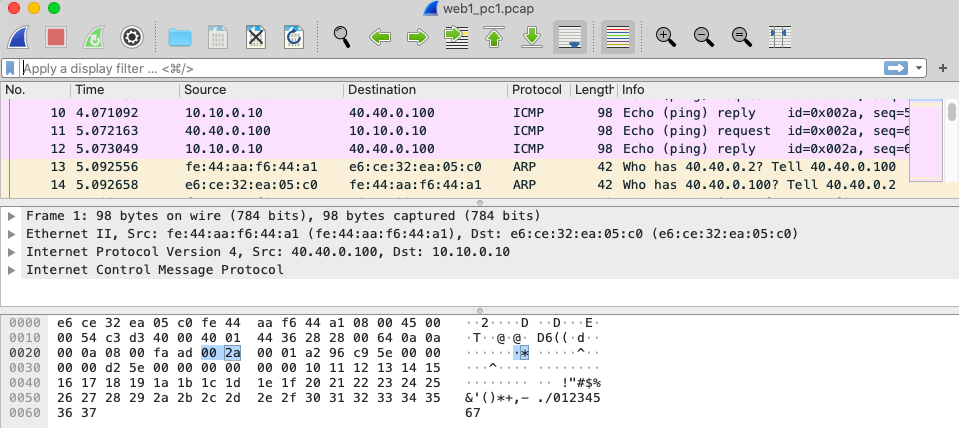
\includegraphics[width=400pt]{Images/web1_pc1_tcpdump.png}
  \caption{Traffic between web1 and pc1 in wireshark}
  \label{fig:2.4.2}
\end{figure}
\subsection{Traffic from web2 to pc2}
Traffic is captured when we ping pc2 from web2 using tcpdump and the .pcap file is imported into the wireshark to display the traffic flow.
\begin{figure}[H]
\centering
  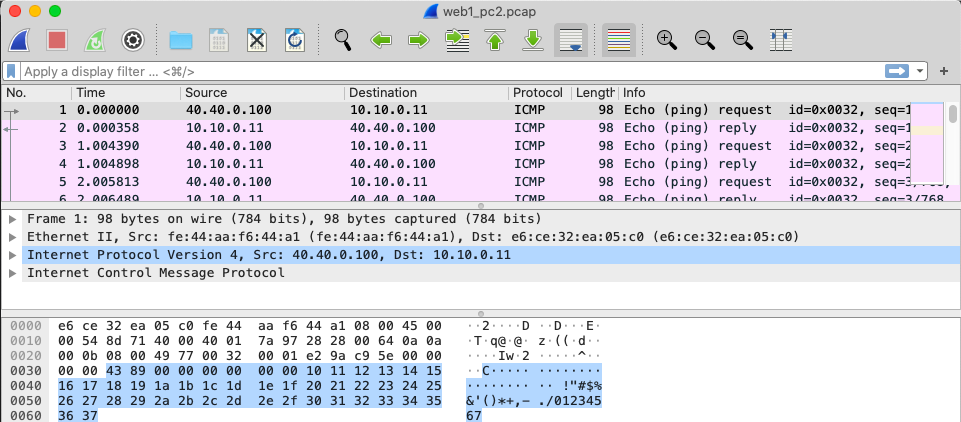
\includegraphics[width=400pt]{Images/web1_pc2_tcpdump.png}
  \caption{Traffic between web2 and pc2 in wireshark}
  \label{fig:2.4.3}
\end{figure}
\subsection{Traffic from pc2 to web2}
Traffic is captured when we ping web2 from pc2 using tcpdump and the .pcap file is imported into the wireshark to display the traffic flow.
\begin{figure}[H]
\centering
  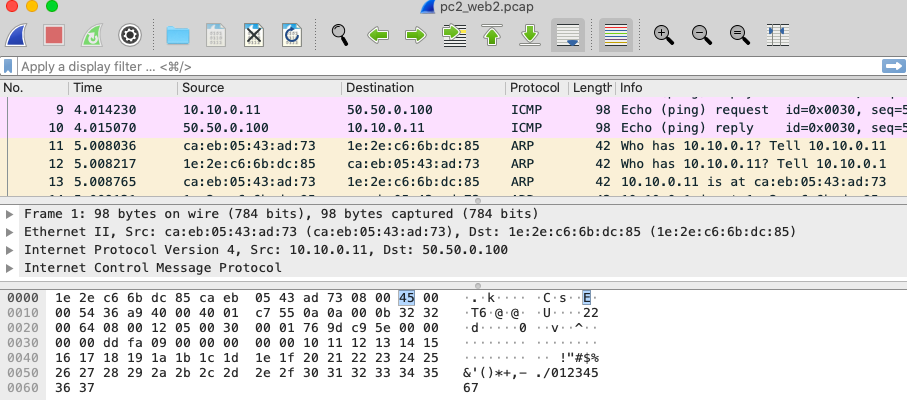
\includegraphics[width=400pt]{Images/pc2_web2_tcpdump.png}
  \caption{Traffic between pc2 and web2 in wireshark}
  \label{fig:2.4.4}
\end{figure}

\section{Checking connectivity between all host}
<<<<<<< HEAD
=======
\newline 1. In this section we are going to check the connectivity between all the hosts.
\newline 2. we cannot reach all the host's due to lack of global connectivity so to provide global connectivity we need to add route entries to every router so that all the networks can communicate with each other.
\subsection{Connectivity between Pc1 and Pc2 and from Pc1 to r1-eth0,r1-eth1,r1-eth2}
we are able to reach from pc1,pc2 and r1 and vice versa because pc1,pc2 and R1 are in the same collision domain.
\begin{figure}[H]
\centering
  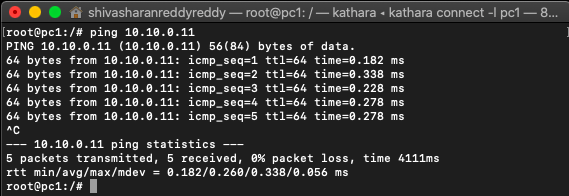
\includegraphics[width=400pt]{Images/Connectivity between Pc1 and Pc2.png}
  \caption{connectivity between pc1 and pc2}
  \label{fig:3.1}
\end{figure}
\begin{figure}[H]
\centering
  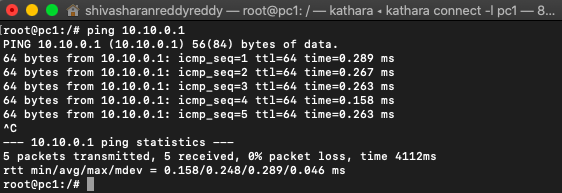
\includegraphics[width=400pt]{Images/Connectivity between Pc1 and R1-eth0.png}
  \caption{connectivity between pc1 and r1-eth0}
  \label{fig:3.1}
\end{figure}
\begin{figure}[H]
\centering
  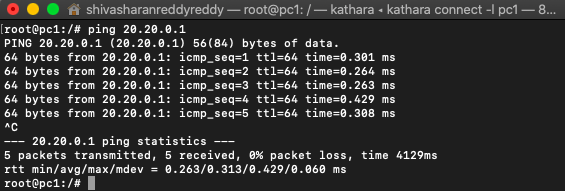
\includegraphics[width=400pt]{Images/Connectivity between pc1 and r1-eth2.png}
  \caption{connectivity between pc1 and r1-eth1}
  \label{fig:3.1}
\end{figure}
\begin{figure}[H]
\centering
  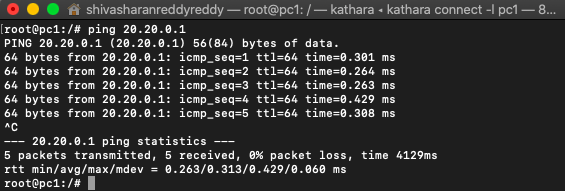
\includegraphics[width=400pt]{Images/Connectivity between pc1 and r1-eth2.png}
  \caption{connectivity between pc1 and r1-eth2}
  \label{fig:3.1}
\end{figure} [H]
\subsection{Connectivity between Pc1 and r2 and r3}
we cannot reach R2 or R3 from pc1,pc2,r1 because they are in the different network and for reaching those network we need to implement global connectivity that is we need to add routing entries in the routers
\newline We need to add a route entry on R1,R2,R3 in order to reach between these host 
\begin{figure}[H]
\centering
  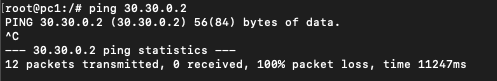
\includegraphics[width=400pt]{Images/connectivity between pc1 and r2.png}
  \caption{R2 is not reachable from PC1 }
  \label{fig:3.1}
\end{figure} [H]
\begin{figure}[H]
\centering
  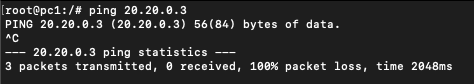
\includegraphics[width=400pt]{Images/connectivity between pc1 and r3.png}
  \caption{R3 is not reachable form pc1}
  \label{fig:3.1}
\end{figure} [H]
\subsection{Connectivity between web1 and r2, web2 and r3}
We will be able to reach these host's because they are in the same collision domain and we have assigned their respective default gateway's.
\begin{figure}[H]
\centering
  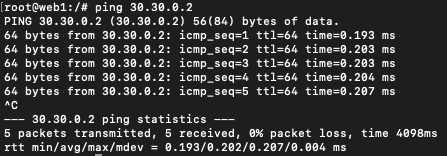
\includegraphics[width=400pt]{Images/Connectivity between web1 and r2.png}
  \caption{connectivity between web1 and r2}
  \label{fig:3.1}
\end{figure} [H]
\begin{figure}[H]
\centering
  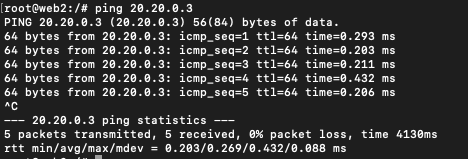
\includegraphics[width=400pt]{Images/Connectivity between web2 and r3.png}
  \caption{connectivity between web2 and r3}
  \label{fig:3.1}
\end{figure} [H]

\section{Capturing the traffic on the collision domains}
In mac OS we cannot find collision domains in the traffic using Wireshark. To capture the traffic, used ping command to connect to between the systems, and ran tcpdump in the background, and redirected the dump to a .pcap file. Later by importing the .pcap into Wireshark we could able to observe the traffic.
\newline Below screenshots displays the traffic captured from different systems at collision domains,
\subsection{Traffic from pc1 to web1}
Traffic is captured when we ping web1 from pc1 using tcpdump and the .pcap file is imported into the wireshark to display the traffic flow.
\begin{figure}[H]
\centering
  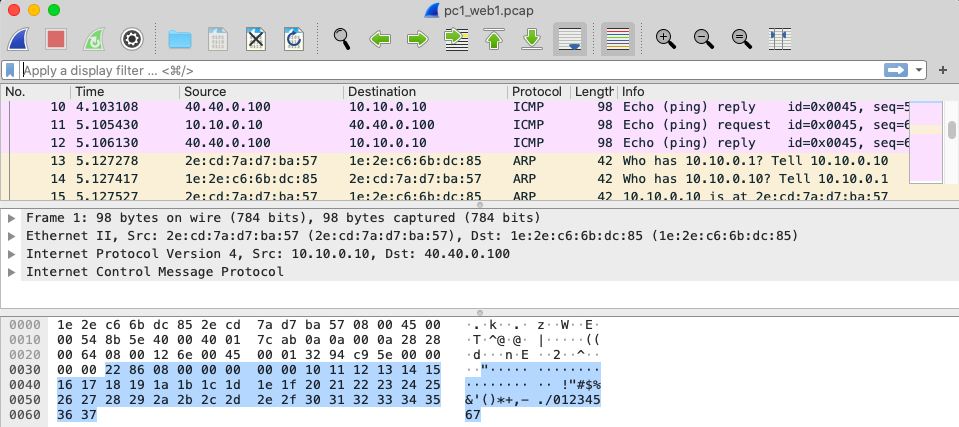
\includegraphics[width=400pt]{Images/pc1_web1_tcpdump.png}
  \caption{Traffic between pc1 and web1 in wireshark}
  \label{fig:2.4.1}
\end{figure}
\subsection{Traffic from web1 to pc1}
Traffic is captured when we ping pc1 from web1 using tcpdump and the .pcap file is imported into the wireshark to display the traffic flow.
\begin{figure}[H]
\centering
  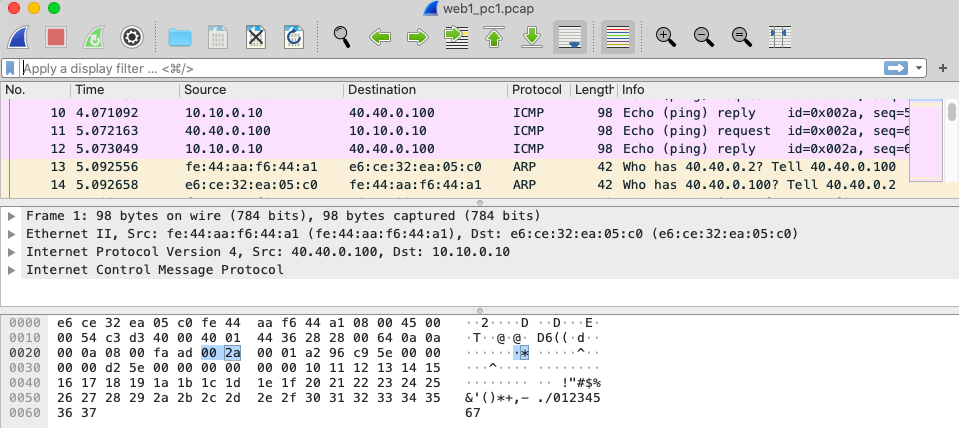
\includegraphics[width=400pt]{Images/web1_pc1_tcpdump.png}
  \caption{Traffic between web1 and pc1 in wireshark}
  \label{fig:2.4.2}
\end{figure}
\subsection{Traffic from web2 to pc2}
Traffic is captured when we ping pc2 from web2 using tcpdump and the .pcap file is imported into the wireshark to display the traffic flow.
\begin{figure}[H]
\centering
  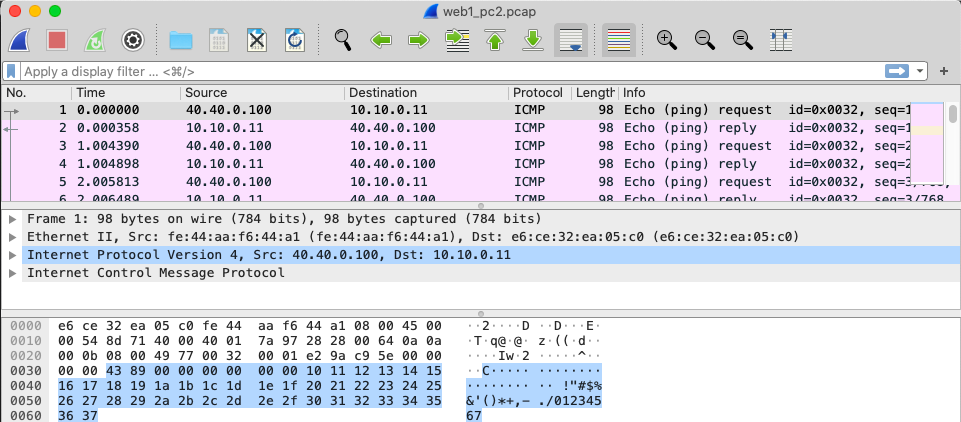
\includegraphics[width=400pt]{Images/web1_pc2_tcpdump.png}
  \caption{Traffic between web2 and pc2 in wireshark}
  \label{fig:2.4.3}
\end{figure}
\subsection{Traffic from pc2 to web2}
Traffic is captured when we ping web2 from pc2 using tcpdump and the .pcap file is imported into the wireshark to display the traffic flow.
\begin{figure}[H]
\centering
  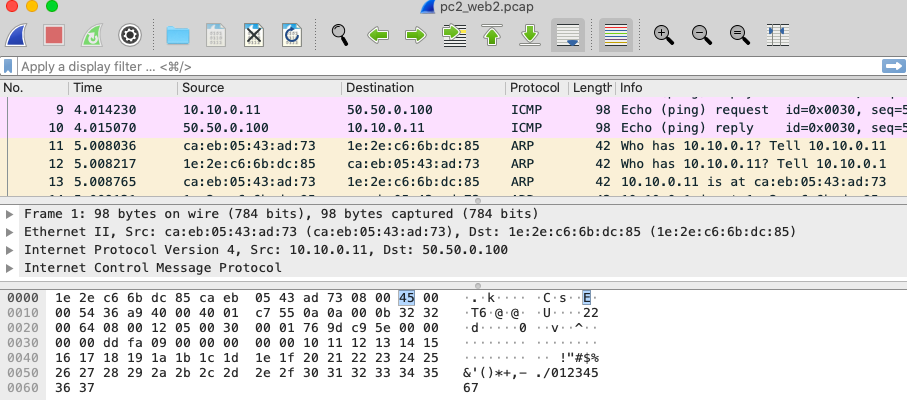
\includegraphics[width=400pt]{Images/pc2_web2_tcpdump.png}
  \caption{Traffic between pc2 and web2 in wireshark}
  \label{fig:2.4.4}
\end{figure}

\section{Checking connectivity between all host}
>>>>>>> 48a684cd851a8df39224f8b6725a51314ead5f6e
1.In this section we are going to check the connectivity between all the hosts.
\newline 2. we cannot reach all the host's due to lack of global connectivity so to provide global connectivity we need to add route entries to every router so that all the networks can communicate with each other.
\subsection{Connectivity between Pc1 and Pc2 and from Pc1 to r1-eth0,r1-eth1,r1-eth2}
we are able to reach from pc1,pc2 and r1 and vice versa because pc1,pc2 and R1 are in the same collision domain.
\begin{figure}[H]
\centering
  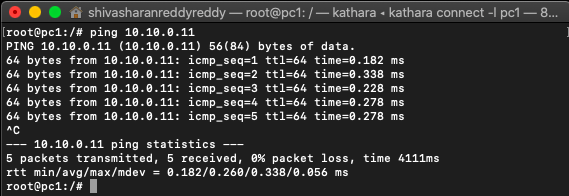
\includegraphics[width=400pt]{Images/Connectivity between Pc1 and Pc2.png}
  \caption{connectivity between pc1 and pc2}
  \label{fig:2.22}
\end{figure}
\begin{figure}[H]
\centering
  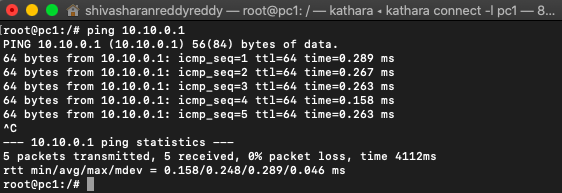
\includegraphics[width=400pt]{Images/Connectivity between Pc1 and R1-eth0.png}
  \caption{connectivity between pc1 and r1-eth0}
  \label{fig:2.23}
\end{figure}
\begin{figure}[H]
\centering
  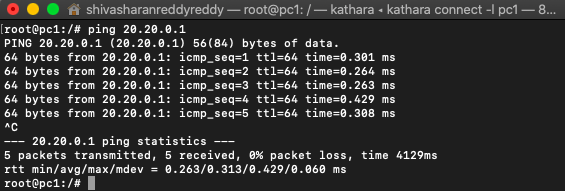
\includegraphics[width=400pt]{Images/Connectivity between pc1 and r1-eth2.png}
  \caption{connectivity between pc1 and r1-eth1}
  \label{fig:2.25}
\end{figure}
\begin{figure}[H]
\centering
  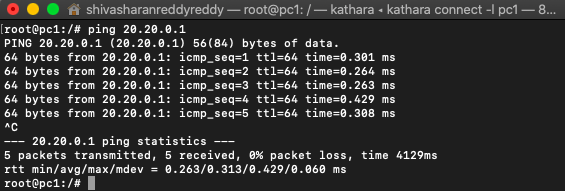
\includegraphics[width=400pt]{Images/Connectivity between pc1 and r1-eth2.png}
  \caption{connectivity between pc1 and r1-eth2}
  \label{fig:2.26}
\end{figure} [H]
\subsection{Connectivity between Pc1 and r2 and r3}
we cannot reach R2 or R3 from pc1,pc2,r1 because they are in the different network and for reaching those network we need to implement global connectivity that is we need to add routing entries in the routers
\newline We need to add a route entry on R1,R2,R3 in order to reach between these host 
\begin{figure}[H]
\centering
  \includegraphics[width=400pt]{Images/connectivity between pc1 and r2.png}
  \caption{R2 is not reachable from PC1 }
  \label{fig:2.27}
\end{figure} [H]
<<<<<<< HEAD
=======
\subsection{Connectivity between Pc1 and r2 and r3}
we cannot reach R2 or R3 from pc1,pc2,r1 because they are in the different network and for reaching those network we need to implement global connectivity that is we need to add routing entries in the routers
\newline We need to add a route entry on R1,R2,R3 in order to reach between these host 
\begin{figure}[H]
\centering
  \includegraphics[width=400pt]{Images/connectivity between pc1 and r2.png}
  \caption{R2 is not reachable from PC1 }
  \label{fig:3.1}
\end{figure} [H]
>>>>>>> 48a684cd851a8df39224f8b6725a51314ead5f6e
\begin{figure}[H]
\centering
  \includegraphics[width=400pt]{Images/connectivity between pc1 and r3.png}
  \caption{R3 is not reachable form pc1}
<<<<<<< HEAD
  \label{fig:2.28}
=======
  \label{fig:3.1}
>>>>>>> 48a684cd851a8df39224f8b6725a51314ead5f6e
\end{figure} [H]
\subsection{Connectivity between web1 and r2, web2 and r3}
We will be able to reach these host's because they are in the same collision domain and we have assigned their respective default gateway's.
\begin{figure}[H]
\centering
  \includegraphics[width=400pt]{Images/Connectivity between web1 and r2.png}
  \caption{connectivity between web1 and r2}
<<<<<<< HEAD
  \label{fig:2.29}
=======
  \label{fig:3.1}
>>>>>>> 48a684cd851a8df39224f8b6725a51314ead5f6e
\end{figure} [H]
\begin{figure}[H]
\centering
  \includegraphics[width=400pt]{Images/Connectivity between web2 and r3.png}
  \caption{connectivity between web2 and r3}
<<<<<<< HEAD
  \label{fig:2.30}
=======
  \label{fig:3.1}
>>>>>>> 48a684cd851a8df39224f8b6725a51314ead5f6e
\end{figure} [H]

\section{Providing global connectivity}
In this section, to provide global connectivity we are going to manually add routing entries into the routing tables of r1, r2, and r3. 
\subsection{Entries into the routing table of r2}
This is achieved using the following commands.
\newline 1) route add -net 10.10.0.0 net mask 255.255.255.0 gw 30.30.0.1 dev eth0
\newline 2) route add -net 50.50.0.0 net mask 255.255.255.128 gw 30.30.0.1 eth0
\begin{figure}[H]
\centering
  \includegraphics[width=400pt]{Images/routing_tableEntries_r2.png}
  \caption{Routing table entries for r2}
  \label{fig:2.6.1}
\end{figure}

\subsection{Entries into the routing table of r3}
This is achieved using the following commands.
\newline 1) route add -net 10.10.0.0 netmask 255.255.255.0 gw 20.20.0.1 dev eth0
\newline 2) route add -net 40.40.0.0 netmask 255.255.255.0 gw 20.20.0.1 eth0
\begin{figure}[H]
\centering
  \includegraphics[width=400pt]{Images/routing_tableEntries_r3.png}
  \caption{Routing table entries for r3}
  \label{fig:2.6.2}
\end{figure}

\subsection{Entries into the routing table of r1}
This is achieved using the following commands.
\newline 1) route add -net 40.40.0.0 netmask 255.255.0.0 gw 30.30.0.2 eth1
\newline 2) route add -net 50.50.0.0 netmask 255.255.240.0 gw 20.20.0.3 eth2
\begin{figure}[H]
\centering
  \includegraphics[width=400pt]{Images/routing_tableEntries_r1.png}
  \caption{Routing table entries for r1}
<<<<<<< HEAD
  \label{fig:2.6.3}
=======
  \label{fig:3.1}
>>>>>>> 48a684cd851a8df39224f8b6725a51314ead5f6e
\end{figure}

\section {Ping from pc1 to web1}
After we successfully provide global connectivity we are able to reach between all the hosts in the given network 
\newline When we ping from pc1 to web1, the packets start from pc1 and reaches r1. We have configured a route in r1 so that the R1 routes forwards packets to r2, once the packet reaches r2 it sends it to web1 because in web1 the default gateway is configures a R2 hence we will be able to ping from pc1 to web1, As shown below.
\begin{figure}[H]
\centering
  \includegraphics[width=400pt]{Images/Connectivity from pc1 to web1.png}
  \caption{connectivity between pc1 and Web1}
<<<<<<< HEAD
  \label{fig:2.31}
=======
  \label{fig:3.1}
>>>>>>> 48a684cd851a8df39224f8b6725a51314ead5f6e
\end{figure}